%!TEX TS-program = lualatex
%!TEX TS-program = pdftex
%!TEX TS-program = xetex
\documentclass[11pt,slovak,twosides,openany]{scrbook}
\usepackage{fontspec}
\setmonofont{Consolas}
\usepackage[a5paper]{geometry}
\geometry{verbose,rmargin=2.3cm}
\usepackage{fancyhdr}
\pagestyle{fancy}
\setcounter{secnumdepth}{3}
\setcounter{tocdepth}{0}
\usepackage{array}
\usepackage{verbatim}
\usepackage{longtable}
\usepackage{graphicx}
% vyzerato tak ze toto nebolo potrebne a len to generovalo error:
%\usepackage{eurosym}
\usepackage{marvosym}
\usepackage[unicode=true]{hyperref}


\makeatletter

%%%%%%%%%%%%%%%%%%%%%%%%%%%%%% LyX specific LaTeX commands.
%% Because html converters don't know tabularnewline
\providecommand{\tabularnewline}{\\}

%%%%%%%%%%%%%%%%%%%%%%%%%%%%%% User specified LaTeX commands.
%%% CONSTANTS
\newcommand{\nadpis}{Matfyzákov sprievodca po~galaxii}
%Otvorenie akademickeho roka den a hodina
\newcommand{\akademickyRok}{2022/2023}
\newcommand{\otvorenieARd}{19. 9. 2022}
% TODO: nenansiel som cas otvorenia AR ale predpokladam ze o 11:00. Na strake upece som nasieil posledne veni sancte z roku 2019, este asi nepridali
\newcommand{\otvorenieARh}{11:00}
\newcommand{\veniSancte}{\textbf{28.9.2022}}
\newcommand{\veniSanctedd}{v stredu}

%%% PACKAGES
\usepackage{booktabs}% for much better looking tables
\usepackage{array}% for better arrays (eg matrices) in maths
\usepackage{paralist}% very flexible & customisable lists (eg. enumerate/itemize, etc.)

%%% HEADERS & FOOTERS
\usepackage{fancyhdr} % This should be set AFTER setting up the page geometry
\pagestyle{fancy} % options: empty , plain , fancy
\renewcommand*{\chapterpagestyle}{fancy}
%\renewcommand{\headrulewidth}{0pt} % customise the layout...
\fancyhf{}
\chead{}
\fancyfoot[LE,RO]{\thepage}
\fancyhead[LE,RO]{\nadpis}
\fancyhead[LO,RE]{\akademickyRok}

%%% ToC (table of contents) APPEARANCE
\usepackage[titles]{tocloft} % Alter the style of the Table of Contents
\renewcommand{\cftsecfont}{\rmfamily\mdseries\upshape}
\renewcommand{\cftsecpagefont}{\rmfamily\mdseries\upshape} % No bold!

% removing space above chapter
\renewcommand*{\chapterheadstartvskip}{\vspace*{0cm}}

% font sizes
\setkomafont{chapter}{\normalfont\bfseries\fontsize{13}{15.5}\selectfont\scshape}
\setkomafont{section}{\normalfont\fontsize{13}{15.5}\selectfont}
\setkomafont{subsection}{\normalfont\bfseries}

\usepackage{longtable}

\makeatother

\usepackage{xunicode}
\usepackage{polyglossia}
\setdefaultlanguage{slovak}
\begin{document}
\title{\nadpis}
\date{\akademickyRok}


\subtitle{Praktické rady a informácie o štúdiu}


\author{Pripravil ŠKAS}


\publishers{
\begin{figure}
\centering{}
\includegraphics[width=0.6\textwidth]{obrazky/fmfi_logo}
\end{figure}
}

\maketitle
%\tableofcontents{}
\tableofcontents

\chapter{Úvod}

Milá matfyzáčka, milý matfyzák,

vitaj na svojej novej Alma mater, na Matfyze! Blahoželáme Ti k~prijatiu
a želáme Ti veľa šťastia v štúdiu na našej fakulte.

Všetci sme raz boli prváci a zápasili sme s problémami, aké môžu stretnúť
aj Teba. Cieľom tejto publikácie je pomôcť Ti zorientovať sa v~škole,
poradiť čo a ako funguje, na koho sa máš obrátiť, kde sa dobre najesť,
požičať si skriptá a pod.

% @julia: toto by som prepisala - neviem o tom, ze by sme mali rozsirenu verziu a ze by sme ju planovali doplnat; link som uz zmenila, bol nespravny
Máme pre Teba aj elektronickú verziu, ktorú nájdeš na ŠKAS stránke%
\footnote{\href{https://zona.fmph.uniba.sk/skas}{\texttt{https://zona.fmph.uniba.sk/skas}}%
}, príp. pomocou QR kódu:

% @julia: snazila som sa uploadnut novy qr kod, ale vzdy mi napisalo "failed" bez ziadnej chybovej spravy
% @andrej: je potrebné, aby si bola prihlásená na stránke sharelatex.com a potom to pôjde :) už som vygeneroval aj nový :)
\begin{center}

\includegraphics[width=0.55\textwidth]{obrazky/qr_code.png}
\par\end{center}

Okrem samotnej príručky nájdeš užitočné informácie aj na stránke špeciálne dedikovanej pre prvákov: \\ \href{http://www.prvaci.matfyzjein.sk}{\texttt{http://www.prvaci.matfyzjein.sk}}

\newpage
\section*{Kto sme?}

ŠKAS - Študentská komora Akademického senátu FMFI UK. Sme študenti, ktorí chcú vo svojom voľnom čase pracovať aj na zlepšení kvality štúdia a~študentského života na fakulte. \\

Členovia ŠKAS sú desiati volení zástupcovia študentov z rôznych stupňov a študijných odborov FMFI, ktorí reprezentujú a hája záujmy študentskej obce v akademickom senáte. Akademický senát FMFI UK je samosprávny zastupiteľský orgán,
ktorý rozhoduje na svojich zasadnutiach o dôležitých otázkach fungovania fakulty. \\

Môžeš sa na nás obrátiť s akýmkoľvek problémom alebo otázkou ohľadom štúdia, takže neváhaj využiť našu spoločnú mailovú adresu: \href{mailto:skas@fmph.uniba.sk}{\texttt{skas@fmph.uniba.sk}} \\

Počas roka máme aj vlastné verejné zasadania, ktorých sa môže zúčastniť každý študent. Miesto a čas konania nájdeš na \href{https://zona.fmph.uniba.sk/skas/%7D%7BŠKAS stránke}. Miesto zasadania býva väčšinou v pavilóne S, kde má ŠKAS svoju miestnosť (pozri mapu na str.\ \pageref{fig:mapa_fmfi}). \\

%\newpage

%Aktuálny zoznam zvolených ŠKASákov na akademický rok \akademickyRok nájdeš na stránke ŠKAS-u: \href{https://zona.fmph.uniba.sk/skas/}{\texttt{zona.fmph.uniba.sk/skas}}.


%	\begin{table}[h!]
%		\centering
		%\resizebox{\textwidth}{!}{%
%			\begin{tabular}{|l|c|c|}
%				\hline
%				Meno a priezvisko 			&  ŠP    							& fakultný mail (@uniba.sk)        						\\
%				\hline
%				Bc. Ivan Agarský$^* $      		&  mINF   							& \href{mailto:agarsky2@uniba.sk}{\texttt{agarsky2}}   	\\
%				\hline
%				Bc. Boris Bobáľ$^* $    	&  mFJF						     	& \href{mailto:bobal4@uniba.sk}{\texttt{bobal4}} 		\\
%				\hline
%				Bc. Martin Csiba$^* $      			&  mBMF					      		& \href{mailto:csiba17@uniba.sk}{\texttt{csiba17}} 		\\
%				\hline
%				Mgr. Barbora Eckerová$^* $      	&  dFSF							   	& \href{mailto:eckerova6@uniba.sk}{\texttt{eckerova6}} 	\\
%				\hline
%				Bc. Erika Lettrichová$^* $  &  mEMM					    		& \href{mailto:lettrichova11@uniba.sk}{\texttt{lettrichova11}} \\
%				\hline
%				Mgr. Samuel Omasta$^* $  	&  dFPL								& \href{mailto:omasta4@uniba.sk}{\texttt{omasta4}} 	\\
%				\hline
%				Bc. Adam Otruba$^* $  	&  mEOM 								& \href{mailto:otruba9@uniba.sk}{\texttt{otruba9}} 	\\
				%\hline
				%Uprázdnený mandát			&		----------- 				&						----------- 					\\
				%\hline
				%Uprázdnený mandát			&		----------- 				&						----------- 					\\
				%\hline
				%Uprázdnený mandát			&		----------- 				&						----------- 					\\
%				\hline
%			\end{tabular}
%	\end{table}




\chapter{Úvodné slovo prodekana pre Bc. a Mgr. štúdium}

Milé študentky, milí študenti!\\

Dovoľte mi srdečne Vás privítať na pôde Fakulty matematiky, fyziky a informatiky Univerzity Komenského v Bratislave, ktorá je jednou z trinástich fakúlt najväčšej a najstaršej univerzity na Slovensku a je uznávanou inštitúciou aj na svetovej úrovni.\\

Naša fakulta spolupracuje na rôznych svetových projektoch. Patrí k vysokým školám s najnižšou nezamestnanosťou absolventov a naši absolventi patria k najlepšie finančne odmeňovaným po nástupe do praxe.\\

Ďakujeme Vám za Vašu dôveru, že ste si spomedzi všetkých možností na štúdium vybrali práve našu fakultu.\\

Uvedomujem si, že prechod na vysokoškolské štúdium môže byť náročný, a preto sa budeme snažiť Vám ho uľahčiť. S dôverou sa môžete obrátiť na Vašich garantov, tútorov, pedagógov, zamestnancov študijného oddelenia alebo aj priamo na mňa s akýmkoľvek problémom. Od Vás len očakávame poctivú prácu a svedomité štúdium, slušný prístup ku všetkým osobám na fakulte a toleranciu voči ostatným.\\

Prajem Vám veľa úspechov v štúdiu a cíťte sa na fakulte dobre.\\

RNDr. Kristína Rostás, PhD.,

prodekanka pre bakalárske a magisterské štúdium

\chapter{Štúdium}

%\begin{comment}
%Tvoje štúdium sa riadi podľa základného predpisu -- Študijného poriadku
%fakulty.
%\end{comment}
%\begin{comment}
%Základný predpis, podľa ktorého sa riadi Tvoje štúdium, je \textbf{Študijný
%poriadok fakulty}.
%\end{comment}



\section{Študijný poriadok fakulty}

Študijný poriadok fakulty (stiahneš na stránke študijného oddelenia%
\footnote{\href{https://zona.fmph.uniba.sk/studenti-a-studium/studijne-oddelenie//}{\texttt{zona.fmph.uniba.sk/studenti-a-studium/studijne-oddelenie/}}%
}) je základný predpis\textbf{, }podľa ktorého sa riadi Tvoje štúdium.
Vrelo Ti odporúčame si ho prečítať, získaš tak ucelenejší prehľad
o pravidlách a organizácii štúdia, než Ti môžeme poskytnúť v~rozsahu
tejto príručky.


\section{Študijné oddelenie}

Všetky potrebné informácie o Tvojom štúdiu, ako aj pomoc s~rôznou
nutnou byrokraciou, Ti isto počas úradných hodín rady poskytnú referentky študijného oddelenia. 

\begin{table}[h!]
\begin{centering}
\begin{tabular}{|c|c|c|}
  \hline
                 &  doobeda    	  & poobede        \\
  \hline
  \hline
    Pondelok     & -----------    & 13:00 -- 15:00 \\
  \hline
    Utorok       & -----------    & 13:00 -- 15:00 \\
  \hline
    Streda       & 9:00 -- 11:30  & 13:00 -- 15:00 \\
  \hline
    Štvrtok      & 9:00 -- 11:30  & -----------    \\
  \hline
    Piatok       &   -----------  & -----------    \\
  \hline

\end{tabular}

\par\end{centering}
\protect\caption{Úradné hodiny študijného oddelenia. Študijné oddelenie číslo dverí 5 má v utorok úradné hodiny doobeda, nie poobede.} %Musis overit
\label{tab:SO-UH}
\end{table}

Študijné oddelenie sa nachádza v~pavilóne matematiky (pozri mapu
na str.\ \pageref{fig:mapa_fmfi}).

Každý študijný program má pridelenú svoju re\-fe\-ren\-tku (pozri
menovky pri dverách). Potrebné tlačivá a potvrdenia nájdeš na~fakultnom
webe\footnote{\href{https://zona.fmph.uniba.sk/sluzby-a-administrativa/tlaciva/}{\texttt{zona.fmph.uniba.sk/sluzby-a-administrativa/tlaciva/}}}. Dôležité oznamy študijného oddelenia nájdeš na nástenke pred študijným oddelením (oznamy o rektorských a dekanských voľnách, oznamy o odborových a prospechových štipendiách) alebo na Facebookovej stránke ,,Študijné oddelenie FMFI UK"\footnote{\href{www.facebook.com/fmphstudijne/}{\texttt{facebook.com/fmphstudijne/}}} \\

V prípade zlej epidemiologickej situácie, Študijné oddelenie poskytovalo služby výhradne telefonicky a mailovou komunikáciou. V tomto prípade je potrebné s referentkami komunikovať prostredníctvom univerzitne pridelenej mailovej adresy (viď strana \pageref{sec:6.1}). 


\section{Harmonogram štúdia}

Slávnostné otvorenie akademického roka\footnote{Účasť na otvorení akademického roku je dobrovoľná.} {\akademickyRok} sa uskutoční {\otvorenieARd} o {\otvorenieARh} v Aule UK (Šafárikovo námestie č. 6, Bratislava).

\begin{longtable}{|>{\centering}p{0.33\textwidth}|>{\raggedright}p{0.59\textwidth}|}
  \hline 
    \multicolumn{2}{|l|}{\textbf{Zimný semester}}\tabularnewline
      \hline 
      2. 9. – 3. 9. 2021       & Zápis študentov v 1. roku Bc. štúdia\tabularnewline
      \hline 
      27. 8. – 17. 9. 2021     & Zápis študentov vo vyššom roku Bc.\ a Mgr.\ štúdia\tabularnewline
      \hline 
      {20. 9. – 17. 12. 2021}  & {Výučba FMFI (13 týždňov)}\footnote{Študenti odborov, ktorí majú výučbu na viacerých fakultách, môžu mať odlišné termíny výučby. \label{fn2}}\tabularnewline
      \hline 
      koniec septembra         & Slávnostná imatrikulácia novoprijatých študentov\tabularnewline
      \hline 
      koniec novembra          & Beánia Matfyzákov\tabularnewline
      \hline 
      december                 & Vianočná kapustnica a punč\tabularnewline
      \hline 
      3. 1. – 11. 2. 2022      & Skúškové obdobie (7 týždňov) \tabularnewline
      \hline 
    \hline 
    \multicolumn{2}{|l|}{\textbf{Letný semester}}\tabularnewline
      \hline 
      14. 2. – 13. 5. 2022     & Výučba FMFI (13 týždňov)$^\ref{fn2}$ \tabularnewline
      \hline 
      14. 4. – 19. 4. 2022     & Rektorské / dekanské voľno (veľkonočné sviatky) \tabularnewline
      \hline 
     % do 19. 2. 2020           & Odovzdanie indexov prvákov na kontrolu ŠO\tabularnewline
     %\hline
      14. 5. – 30. 6. 2021      & Skúškové obdobie (6 týždňov a 4 dni)\tabularnewline
      \hline 
      júl & Podávanie žiadostí o ubytovanie\tabularnewline
    \hline
\end{longtable}


\section{Dĺžka štúdia}

Štandardná dĺžka štúdia na našej fakulte sú 3 roky pre bakalárske študijné programy, resp. 4 roky pri tzv. konverzných študijných programoch (FYZ, OZE, TEF, DAV a BIN) a 2 roky pre~magisterské štúdium, resp. 3 roky pre konverzné magisterské študijné programy (napr. učiteľské ŠP, MPG, INF a AIN). Prekročenie štandardnej dĺžky štúdia je spoplatnené školným.

Štúdium je možné (podľa Študijného poriadku fakulty) prerušiť naj\-viac
na 1 rok, pri závažných dôvodoch naj\-viac na~2 roky a pri~rodičovskej
dovolenke najviac na 3 roky. Avšak na dané obdobie strácaš štatút študenta.


\section{Kreditový systém}

Kre\-di\-tový systém štúdia využíva zhromažďovanie a prenos \emph{kre\-di\-tov}
(napr. medzi fakultami či univerzitami). Kredity sú číselné hodnoty
priradené k~predmetom, vyjadrujúce množstvo práce potrebnej na ich
absolvovanie. \\

Priemerná záťaž študenta za~celý akademický rok je 60 kreditov,
za semester 30 kreditov. Maximálna záťaž v jednom roku je 90 kreditov
(výnimky s povolením dekana). Študent získava kredity po úspešnom absolvovaní predmetu (t.j. po obdržaní hodnotenia A až E). Počet získaných kreditov za predmet nie je závislý od získaného hodnotenia. \\

Na úspešné ukončenie trojročného bakalárskeho štúdia potrebuješ získať
180 kreditov (240 kreditov v prípade konverzných ŠP). V prípade dvojročného magisterského štúdia je to 120 (resp. 180) kreditov.

\section{Kontrolné etapy štúdia}

Na konci prvého (zimného) semestra je potrebné, aby si získal minimálne \textbf{20 kreditov} za úspešne absolvované predmety. Minimálny počet získaných kreditov, reprezentujúci tzv.\ mi\-ni\-málne tempo štúdia, je \textbf{40 kreditov} za~akademický rok s výnimkou prípadu, že študentovi ostáva vykonať len štátnu skúšku.

\section{Zápis predmetov}

Každý študijný program má svoj \textbf{odporúčaný študijný plán},
v~ktorom je pre~každý semester uvedený zoznam povinných (\textbf{A}), povinne
voliteľných (\textbf{B}) a výberových (\textbf{C}) predmetov. Štandardne si zapisuješ predmety
podľa tohto plánu. Všetky plány sú prístupné na stránke fakulty%
\footnote{\href{https://zona.fmph.uniba.sk/studenti-a-studium/studijne-programy/}{\texttt{zona.fmph.uniba.sk/studenti-a-studium/studijne-programy/}}%
}, kde nájdeš štruktúru (osnovu) predmetov, ich hodnotenie, zoznam prerekvizít, dokonca sylaby štátnych skúšok. 

Okrem prezretia  informačných listov Ti zároveň odporúčame zúčastniť sa prvých prednášok, na ktorých je vyučujúci povinný Ťa oboznámiť s východiskovou literatúrou, sylabami predmetu, prezenciou a hodnotením.

V~prípade záujmu si môžeš zapísať aj predmety určené pre~iný rok
štúdia či z~iných študijných programov. Pred zápisom takýchto predmetov
Ti ale odporúčame pozrieť si ich prerekvizity a konzultovať náročnosť
s~tútorom či samotným učiteľom. \\

Môžeš si zapísať aj \textbf{mimofakultné predmety} v~rámci UK či
inej univerzity. V~prvom rade sa ale treba dohodnúť s~príslušným
učiteľom. Kvôli prenosu kreditov treba následne komunikovať s prodekanmi
pre bakalárske a magisterské štúdium oboch fakúlt -- mali by podpísať tlačivo
„Zmluva o~štúdiu“. \\

Samotný zápis predmetov (na celý akademický rok) prebieha elektronicky
cez akademický systém AiS2, resp. cez VOTR. Na~študijnom oddelení Ti následne vystavia protokol o študijnom pláne. Prvé dva týždne každého semestra je možné zmeniť si už zapísané predmety z dôvodu napr.\ kolízie v rozvrhu.

\section{Absolvovanie predmetov}

Predmet sa považuje za úspešne \emph{absolvovaný}, ak splníš aspoň minimálne kritériá
na jeho splnenie. To znamená, že musíš z~neho dosiahnuť hodnotenie známkou A až E. Zároveň študent získa kredity len za úspešne absolvované predmety.

Hodnotenie predmetov sa spravidla skladá z~hodnotenia za~semester
a z~hodnotenia záverečnou skúškou. Niektoré predmety sú hodnotené
len jednou z~týchto zložiek. \\

Základné pravidlo je, že za svoje štúdium musíš absolvovať všetky
povinné a výber z povinne voliteľných predmetov podľa pravidiel určených
študijným programom (väčšinou treba nazbierať určitý počet kreditov
zo~skupiny predmetov). \\

Ak sa Ti nepodarí úspešne absolvovať povinný predmet, musíš si ho znova zapísať.
Povinne voliteľný predmet si môžeš aj nahradiť. Výberové predmety
nie je potrebné opakovať; ak sa tak ale rozhodneš, musíš ich úspešne
absolvovať. \\

V rámci skúškového obdobia máš okrem štandardného termínu skúšky nárok
aj na~dva \textbf{opravné termíny}, ak spĺňaš podmienky priebežného hodnotenia predmetu (podmienky si určuje každý vyučujúci sám). Pri~\textbf{opakovanom} zápise predmetu máš nárok taktiež na \textbf{dva} opravné termíny.

\section{Preukaz študenta (karta ISIC)}

Preukaz študenta je kombinovaný s~kartou ISIC. Jednu kartu tak používaš
ako preukaz študenta, preukaz do~Univerzitnej / fakultnej knižnice, električenku, zľavu a peňaženku v~internátnych jedálňach a pod. Ku ISIC-u sa viaže množstvo zliav, preto ak plánuješ niekam cestovať, navštíviť kino, nakupovať, atď., nezabudni sa dopredu informovať
o~výhodách na stránke \href{http://www.isic.sk}{\texttt{isic.sk}}.

\section{Knižnice a copycentrá}

\textbf{Fakultná knižnica so študovňou} sa nachádza na -1. poschodí pavilónu
informatiky (pozri mapu na str.\ \pageref{fig:mapa_fmfi}). Prezenčné
knihy môžeš študovať v študovni alebo si ich môžeš vypožičať na večer, či víkend.
Ostatné knihy si môžeš požičať až na~120~dní. 

Ak potrebuješ knihu na obdobie dlhšie ako 120 dní, môžeš si výpožičnú dobu predĺžiť ešte 2-krát (dovedna máš k dispozícii až jeden technický rok). Môžeš tak urobiť prostredníctvom online katalógu Knižničného systému Akademickej knižnice UK\footnote{\href{http://alis.uniba.sk:8088}{\texttt{alis.uniba.sk:8088}}%
}, osobne, písomne (mailom\footnote{\href{mailto:kniznica@fmph.uniba.sk}{\texttt{kniznica@fmph.uniba.sk}}}) alebo telefonicky.

Knižnicu nájdeš aj na FB\footnote{\href{https://www.facebook.com/kniznicafmfi}{\texttt{facebook.com/kniznicafmfi}}}, kde pravidelne informujú o rôznych podujatiach zo sveta vedy, ktoré by študentov mohli zaujímať. Tiež im môžeš zanechať správu na FB a radi Ti pomôžu.\\

Knihy ku konkrétnemu predmetu si môžeš vyhľadať v online katalógu podľa krátkeho kódu predmetu (napr. 1-INF-210) či podľa autora alebo názvu knižky. Ak je kniha vypožičaná, môžeš si ju pomocou online katalógu vyžiadať (tzv. žiadankou), čím sa skráti výpožičná lehota tomu, kto ju má požičanú a kniha Ti bude k dispozícii spravidla do 7 dní. Keď ju študent vráti, Tebe príde automaticky mail, že je pripravená v knižnici. Treba si ju vyzdvihnúť do 7 dní. Video sprievodcu knižnicou a knižničným systémom môžeš nájsť na linke \href{http://video.matfyzjein.sk/kniznica}{\texttt{video.matfyzjein.sk/kniznica}}}. \\ %
}%príp. pomocou QR kódu:

%\begin{center}
%	\vspace{-0.1cm}
%	
\includegraphics[width=0.4\textwidth]{obrazky/qr_code_LIB.png}
%	\par\end{center}

Na blížiaci sa koniec výpožičnej lehoty Ťa upozorní e-mail na Tvoju univerzitnú adresu (viac sa o nej dočítaš v sekcii \ref{sec:6.1}). Je dôležité vracať knihy načas. Okrem toho, že tak pomôžeš spolužiakom sa ku knihe dostať, vyhneš sa aj poplatkom za omeškanie. Pokuta nie je zanedbateľná, a to 50 centov za knihu za deň. \\

Ako študent UK máš prístup k elektronickým študijným materiálom, k externým informačným zdrojom - databázam, článkom atď. Všetky informácie nájdeš na stránke\footnote{\href{https://zona.fmph.uniba.sk/sluzby-a-administrativa/kniznicne-sluzby/}{\texttt{zona.fmph.uniba.sk/sluzby-a-administrativa/ kniznicne-sluzby/}}} alebo priamo v knižnici, kde vždy nájdeš najnovšie informácie. Zároveň si môžeš požiadať aj o vzdialený prístup a študovať materiály z pohodlia domova. \Smiley

\begin{table}[h!]
\begin{centering}
\begin{center}
\begin{tabular}{|c|c|}
\hline 
Po - Štv & 8:30 -- 15:00 \tabularnewline
\hline 
Pia     & 8:30 -- 13:00 \tabularnewline
\hline
\end{tabular}
\par\end{center}

\par\end{centering}
\protect\caption{Otváracie hodiny knižnice počas akademického roka (od 1.9 - 30.6). Každý posledný piatok v mesiaci je knižnica zatvorená z~dôvodu sanitárneho dňa.}
\label{tab:uradne_hodiny}
\end{table}

Ak si potrebuješ nejakú knižku vypožičať/pozrieť i počas leta (napr. kvôli bakalárke), knižnica je otvorená od pondelka do piatku od 8:30 do 12:30.\\

\noindent
V knižnici sa nachádza aj samoobslužná kopírka/tlačiareň na~mince s\,cenou 5 centov za~stranu A4. Toto zariadenie je napojené na~PC, v~ktorom nájdeš vzorové tlačivá niektorých potvrdení a žiadostí. Možná je aj tlač z~USB kľúča alebo po prihlásení priamo zo súborov uložených na Tvojom fakultnom konte.

Niektoré skriptá sa dajú zakúpiť v~copycentre \textbf{PACI} na~Prírodovedeckej
fakulte. Môžeš si tu nechať aj zviazať svoju prácu. Ďalšie copycentrá
nájdeš na internátoch a v Cubicone.

\begin{comment}
Rôzne skriptá môžeš nájsť a následne si aj vziať v \textbf{skriptárni}, t.j. na označenej poličke pred knižnicou, kde môže ktokoľvek pre druhého študenta zanechať svoje už nepotrebné skriptá.
\end{comment}

Knižnica v \textbf{Centre vedecko-technických informácií}%
\footnote{\href{http://www.cvtisr.sk/}{\texttt{cvtisr.sk}}%
} sa nachádza blízko zastávky \emph{Patrónka}. Za malý ročný poplatok máš prístup k veľkému množstvu publikácií, skrípt a pomocou vzdialeného prístupu do e-zdrojov sa môžeš dostať k rôznym zahraničným článkom. Ak knižku nenájdeš vo fakultnej knižnici, pravdepodobne sa bude dať požičať tu.

Na Michalskej ulici sa nachádza \textbf{Univerzitná knižnica}%
\footnote{\href{http://www.ulib.sk/sk/}{\texttt{ulib.sk/sk/}}%
}. Je to najstaršia a najväčšia vedecká knižnica v Slovenskej republike.
Knihy sa v nej objednávajú pomocou internetového katalógu. 

\section{Mobilita}

Počas štúdia môžeš absolvovať zahraničný študijný pobyt alebo stáž.
Veľmi rozšírený program v rámci EÚ, umožňujúci obe formy, je program
\textbf{Erasmus}, resp. \textbf{Erasmus+}. Ďalej je tu \textbf{Národný štipendij\-ný program},
granty na~základe bilaterálnych dohôd či granty zo~súkromného sektora.
Viac informácií nájdeš na~stránkach fakulty alebo agentúry SAIA\footnote{\href{https://www.saia.sk}{\texttt{www.saia.sk}}%
}.

Vďaka mobilite môžeš študovať či pracovať v zahraničí, ale najmä získať
nové skúsenosti a priateľstvá, zlepšiť sa v cudzom jazyku (zväčša
v angličtine), či spoznať novú kultúru.

\section{Štipendiá}

Štipendiá sa riadia zákonom o vysokých školách, ktorý dopĺňa \textbf{Štipendijný
poriadok fakulty\footnote{\href{https://zona.fmph.uniba.sk/fileadmin/fmfi/fakulta/legislativa/Stipendijny_poriadok_FMFI_UK_uplne_znenie_jun2020.pdf}{\texttt{zona.fmph.uniba.sk/fileadmin/fmfi/fakulta/legislativa/\-Stipendijny\_poriadok\_FMFI\_UK\_uplne\_znenie\_jun2020.pdf}}}}. Tam sú uvedené aj konkrétne kri\-té\-riá ich prideľovania. Štipendiá sa rozdeľujú na motivačné, odborové a sociálne. 

\subsection{Motivačné štipendium}

Motivačné štipendium sa udeľuje za~vynikajúci prospech (\emph{prospechové štipendium}) alebo za mimoriadne výsledky (\emph{mimoriadne štipendium}).

\subsubsection{Prospechové štipendium}
Prospechové štipendium je priznávané 10\% študentov (tvoria sa 2 poradovníky: pre prvákov a pre druhákov a vyššie roky štúdia). Na to, aby si ako prvák dostal v letnom semestri prospechové štipendium, musíš splniť nasledujúce podmienky: 

	\begin{enumerate}
		\itemsep0em 
		\item vo všetkých zapísaných predmetoch za zimný / letný semester si získal hodnotenie A až E, 	
		\item dosiahol si vážený študijný priemer menší alebo rovný 1,30,
		\item a získal si najmenej 27 kreditov za semester.
	\end{enumerate}

\subsubsection{Mimoriadne štipendium}

Mimoriadne štipendium je udeľované za dosiahnutie vynikajúceho výsledku v oblasti štúdia, výskumu, vývoja, umeleckej alebo športovej činnosti.

\subsection{Odborové štipendium}

Odborové štipendium sa udeľuje časti študentov\footnote{50\% študentov 1. ročníka Bc. a vo vyšších ročníkoch je odborové štupendium priznané 30\% študentom} na študijných odboroch podporovaných Ministerstvom školstva, vedy, výskumu a športu SR (všetky odbory na FMFI UK sú podporované). 

\subsection{Sociálne štipendium}

Sociálne štipendium môže byť priznané iba tým študentom, ktorých rodinné príjmy sa približujú sumám životného minima. Posudzovať sa môžu príjmy Tvojich rodičov, súrodencov, manžela/manželky, príp. vlastných detí - teda najbližší rodinní príslušníci. Posudzuje sa vždy aktuálna situácia v čase podania žiadosti. Ak je štipendium priznané, vypláca sa v mesačných čiastkach od mesiaca, v ktorom bola žiadosť podaná. \\

Sociálne štipendiá má vo svojej agende p. Mináriková\footnote{\href{mailto:Maria.Minarikova@fmph.uniba.sk}{\texttt{Maria.Minarikova@fmph.uniba.sk}}} (dvere č.4) a motivačné, odborové, prospechové štipendiá rieši p. Majerčíková\footnote{\href{mailto:Emilia.Majercikova@fmph.uniba.sk}{\texttt{Emilia.Majercikova@fmph.uniba.sk}}} (dvere č.2) .\\

Viac informácií ohľadom štipendií nájdeš na stránke\footnote{\href{https://zona.fmph.uniba.sk/studenti-a-studium/stipendia/}{\texttt{zona.fmph.uniba.sk/studenti-a-studium/stipendia/}}} alebo u svojej študijnej referentky.

\newpage
\section{Študentská pôžička}

V prípade potreby môžeš požiadať o študentskú pôžičku z Fondu na podporu
vzdelávania vo výške až 5 000 € (pre doktorandov 8 000 €) na akademický
rok. Splátky s úrokom vo výške 3\% sa začnú až po skončení štúdia.
Lehota splatnosti je najviac 10 rokov. Viac sa dozvieš na \href{http://www.fnpv.sk}{\texttt{fnpv.sk}}.


\chapter{Práva a povinnosti študenta}

Je veľmi dobré a užitočné poznať svoje práva a povinnosti. V~prípade
štúdia na vysokej škole sú ich hlavnými zdrojmi:
\begin{enumerate}
\itemsep0em
\item zákon č. 131/2002 Z. z. o vysokých školách v znení neskorších predpisov,
\item Študijný poriadok fakulty a
\item smernice rektora univerzity či dekana fakulty.
\end{enumerate}
Odporúčame Ti prečítať si ich, my spomenieme len niektoré informácie
z~nich.


\section{Práva}

Medzi základné práva patrí právo študovať študijný program, na~ktorý
si bol(a) prijatý(á). Svoj študijný plán si môžeš v~medziach študijného
programu vytvoriť podľa svojho uváženia. \\

V~rámci svojho štúdia sa môžeš zároveň uchádzať aj o~štúdium na
inej vysokej škole, a to aj v~zahraničí. \\

Svoj názor nielenže môžeš slobodne prejaviť, ale dokonca budeme radi,
ak sa oň podelíš v \textbf{študentskej ankete} (pozri \ref{subsec:4.1.1}). Otázky, sťažnosti či pripomienky ohľadne Bc. a Mgr. štúdia môžeš napísať do~\textbf{čiernej skrinky} (pozri \ref{subsec:4.1.2}), ktorú nájdeš v AiSe. Vedenie fakulty si veľmi váži dobre mienenú (konštruktívnu) kritiku, snahu študentov o~akékoľvek zlepšenia
a pokiaľ je to možné, vyjde v~ústrety. \\

Ak si myslíš, že došlo k~porušeniu Tvojich práv, môžeš sa obrátiť v nasledujúcom poradí
 na viacero osôb. V~prvom rade sa snaž problém vyriešiť 
tam, kde vznikol (napr.\ priamo s~vyučujúcim). V~prípade neúspechu 
sa môžeš obrátiť na tútora alebo garanta študijného programu, potom na nás (ŠKAS) alebo na\emph{~prodekanku pre bakalárske a magisterské 
štúdium}. Poslednou inštanciou, na koho sa možno na fakulte obrátiť, je dekan.


\subsection{Študentská anketa} \label{subsec:4.1.1}

Už niekoľko rokov prebieha na fakulte na konci každého semestra (a počas skúškového obdobia) študentská anketa.
Študenti v~nej môžu \textbf{anonymne} vyjadriť svoj názor na~výučbu, celkový chod fakulty 
či technické vybavenie na~fakulte. \\

Študentskú anketu berie vedenie fakulty veľmi vážne. Snaží sa riešiť
problémy, na~ktoré študenti poukazujú. Preto Ti odporúčame zúčastniť
sa jej a pomôcť tak v~zlepšovaní kvality štúdia na našej fakulte. \\

Po skončení ankety vedenie uverejňuje tzv \emph{Stanovisko vedenia}, v ktorom sa snažia odpovedať na frekventované komentáre vo \emph{všeobecných otázkach}. Taktiež sa má možnosť vyjadriť učiteľ predmetu, či garant ku svojmu \emph{predmetu} alebo \emph{študijnému programu}. Výsledky ankety sa dajú využiť aj pri výbere predmetov. Po prihlásení
sa na stránke ankety uvidíš názory študentov na~kvalitu či obtiažnosť predmetov a ich odporúčanie, či si daný predmet zapísať, alebo nie. \\

Anketa sa nachádza na adrese \href{https://anketa.fmph.uniba.sk}{\texttt{anketa.fmph.uniba.sk}}.

\subsection{Čierna skrinka} \label{subsec:4.1.2}

Čierna skrinka je miesto pre otázky či pripomienky týkajúce sa
štúdia. Môžeš do nej anonymne alebo pod svojím menom napísať a na rovnakom mieste sa Ti bude
snažiť odpovedať prodekanka pre bakalárske a magisterské štúdium. Prosíme Ťa, nezneužívaj Čiernu skrinku ako ,,informačný kanál", na niektoré otázky Ti vieme odpovedať aj my \Smiley.\\

Nápady a potrehy, za ktoré sa nie je potrebné skrývať za rúšku anonymity, posielaj prodekanke pre bakalárske a magisterské štúdium mailom na: 

\begin{center}
\href{mailto:kristina.rostas@fmph.uniba.sk}{\texttt{kristina.rostas@fmph.uniba.sk}}
\end{center}

Čierna skrinka je prístupná cez AIS%
\footnote{\href{https://ais2.uniba.sk}{\texttt{ais2.uniba.sk}}%
} dvomi spôsobmi: 
\begin{enumerate}\setlength\itemsep{1pt}
\item Cez menu vľavo Administratívny systém > Diskusia k téme 
\item Cez oznam \textquotedbl{}Diskusie\textquotedbl{} v pravom stĺpci na
úvodnej stánke
\end{enumerate}

\subsection{FB stránka a skupina, YouTube kanál a Instagram}


%https://www.facebook.com/MatFyzJeIn/
K oficiálnym komunikačným médiam našej fakulty patrí Facebookova stránka \href{https://www.facebook.com/MatFyzJeIn/}{\texttt{MatFyzJeIn}} na ktorej nájdeš aktuálne udalosti na fakulte, eventy, informácie o úspechoch našich študentov a pedagógov a pod. Tiež odporúčame sledovať Facebookovu stránku \href{https://www.facebook.com/matfyzjobs/}{\texttt{matfyzjobs}}, na ktorej nájdeš uverejňované ponuky prevažne od absolventov našej fakulty.\\ 

V roku 2020 vznikla neformálnejšia Facebookova skupina s cieľom komornejšej komunikácie študentov, absolventov a priaznivcov MatFyzu. Tú nájdeš pod názvom ,,\emph{Fakulta matematiky, fyziky a informatiky - FMFI UK BA}". \\

Zaujímavé prednášky, video rozhovory a populárno-vedecké videá môžeš sledovať na YouTube
kanáli našej fakulty {\href{http://www.youtube.com/MatFyzJeIn}{\texttt{youtube.com\ /MatFyzJeIn}}%
}. \\

Ako ďalší zdroj informácií Ti môže poslúžiť aj fakultný Instagram @matfyjein. 
%K neformálnejším zdrojom informácii patria \href{http://blog.matfyz.sk}{\texttt{blog.matfyz.sk}}
%a \href{http://wiki.matfyz.sk}{\texttt{wiki.matfyz.sk}}. Na blogu si môžeš
%prečítať články ostatných študentov a na wiki nájsť rôzne informácie,
%ktoré študenti pokladali za užitočné. Informácie o prebiehajúcich
%podujatiach a novinkách, týkajúcich sa študentov nájdeš najmä na Facebookovej
%stránke\footnote{\href{https://www.facebook.com/MatFyzJeIn}{\texttt{facebook.com/MatFyzJeIn}}%
%}.



\section{Povinnosti}

Povinnosťou nás, študentov, je okrem snahy naučiť sa čo najviac aj
dodržiavanie vnútorných predpisov univerzity a fakulty. Medzi tieto
povinnosti patrí aj ochrana nášho spoločného majetku a dobrého mena
školy. V~prípade porušenia právnych predpisov alebo vnútorných predpisov
sa môžeš dostať aj pred \textbf{disciplinárnu komisiu} fakulty.\\

Všetky svoje práva a tiež povinnosti nájdeš \textbf{\href{https://zona.fmph.uniba.sk/fileadmin/fmfi/fakulta/legislativa/Studijny_poriadok_FMFI_UK_maj2020.pdf}{Študijnom poriadku fakulty}}, konkrétne čl. 2.


\chapter{Dianie na fakulte}

\section{Voľný čas na fakulte}

Počas teplejších dní môžeš ísť von do \textbf{Relaxu}. Na vrátnici
v~pavilóne matematiky Ti požičajú aj hojdacie siete, bedmintonové
rakety alebo discgolgové taniere, ktoré môžeš použiť na
\textbf{discgolfovom ihrisku} rozpriesterajúcom sa v okolí fakulty. Rovnako si môžeš požičať aj fixky na exteriérovú tabuľu.\\


Ako si si mohol počas svojho krátkeho času na MatFyze všimnúť, pri matematickej vrátnici (pod študijným oddelením, pozri mapu na str. \pageref{fig:mapa_fmfi}) vznikol v spolupráci s partnermi z praxe nový priestor na trávenie voľné času – UniSpace.\\

\textbf{Unispace} Ti poslúži kedykoľvek a v každom počasí, bude vybavená kaviarňou (s posedením), uzamykateľnými skrinkami, tromi ,,mítingovkami", relax a study zónou, pódiom na eventy, spoločenskými hrami a dokonca \textbf{funkčným klavírom} (slúchadlá k nemu si môžeš vypožičať na vrátnici). Ak chceš hrať bez slúchadiel, vždy musíš brať ohľad na ostatných ľudí v miestnosti, a študijné oddelenie nad~Tebou. Môžeš si v nej dobiť notebook alebo mobil (ak máš nabíjačku). V miestnosti taktiež nájdeš aj Wi-Fi. Ak sa nebudú v priestore konať žiadne eventy, priestor bude určený na štúdium a prácu pre študentov našej fakulty. \\

Pravidelne sa v nej budú konať eventy (semináre, workshopy) spoločností previazaných s praxou. Taktiež môžeš so spolužiakmi medzi vyučovaním používať \textbf{pingpongový stôl} za UniSpace-om, rakety a loptičky sa opäť požičiavajú na~vrátnici.

Ďalšou oddychovou miestnosťou bude \textbf{Vacuum lounge}. Nájdeš ju pri spojovacej chodbe medzi pavilónom posluchární a pavilónom fyziky (viď. mapu na str. \pageref{fig:mapa_fmfi}). V miestnosti nájdeš miesto na prácu s kapacitou cca 20 študentov, pohodlné gauče, tulivaky,  premietacie plátno s projektorom a klimatizáciu. Miestnosť bude primárne určená ako study zóna, v ktorej pravidelne bude spoločnosť Vacuumlabs (spolu s partnermi) organizovať workshopy, výstavy a pod. V ostatnom čase Ti bude plne k dispozícii na štúdium a trávenie času medzi prednáškami.\\

Za posluchárňou A sa nachádza priestor s tromi umiestnenými hojdacími sieťami a pohodlným gaučom. V pavilóne fyziky tiež nájdeš novovybudovanú oddychovo-pracovnú zónu so stolíkmi, zásuvkami a kreslami. Nachádza sa pri F1 246.\\

Na oddych ti bude slúžiť aj priestor pod schodiskom neďaleko miestnosti M-VII. Okrem stolov na štúdium pred prednáškou či cvičením v ňom nájdeš aj barové stoličky, či pohodlný gauč. \\

\textbf{Pavilón S} je pavilón športu na našej fakulte. Odohráva sa tu časť výuky telesnej výchovy. Nájdeš tu napr. ping-pongové stoly, bedmintonové /volejbalové ihrisko, lezeckú stenu, posilňovňu či dokonca aj saunu. Na poschodí sa nachádza miestnosť na jógu a nové sídlo ŠKASu. V prípade návštevy pavilónu mimo hodín telesnej výchovy platí nepísané pravidlo, že študenti majú zväčša vyhradené doobedné hodiny a zamestnanci poobedné hodiny. Treba sa však dohodnúť osobne alebo na tel. čísle 02/60295110 (klapka 110). %Lezecká stena mimo vyučovacích hodín prístupná nie je.

Voľné miestnosti na učenie či trávenie voľna so spolužiakmi môžeš
nájsť na~stránke \href{https://candle.fmph.uniba.sk}{\texttt{candle.fmph.uniba.sk}}. 


\section{Podujatia}

Počas roka sa na Matfyze okrem odborných podujatí odohrávajú aj oddychové
aktivity. V priebehu roka ŠKAS organizuje rôzne prednášky, napr. (prednáška Čo je to realita?, Karierny workshop, Time management atď.) \\

Obvykle sa koncom novembra koná \textbf{Beánia matfyzákov}. Ide o
spoločenskú udalosť, kde Ťa okrem prijímania novozapísaných študentov čaká kultúrny program, hudba a zábava.\\

V decembri organizujeme \textbf{Vianočný matfyzácky punč a kapustnicu}.
Táto akcia, ktorá sčasti oslavuje blížiaci sa koniec zimného semestra,
má aj príjemnú predvianočnú atmosféru.\\


Na Matfyze funguje taktiež iniciatíva \textbf{Život po matfyze}, ktorej členovia v priebehu roka organizujú rôzne spoločenské a edukačné aktivity. 

% @julia: toto je tiez zaujimava info :D mali by sme to organizovat?
% @andrej: o tom nič neviem a radšej by som to sem nedával, pretože potom by to mala byť pre nás už povinnosť :D
%Počas jari sme v posledných rokoch organizovali podujatie\textbf{
%Matfyz ožíva}, kde sa študenti môžu stretnúť s vedením a zamestnancami
%fakulty. Ponúka priestor pre rozhovory, hry, šport a naviac môžeme
%skrášliť naše fakultné prostredie. V~rámci nej vznikol aj levanduľový
%nápis pri soche Kopernika, vznikol priestor Relax a v ňom pribudli
%laná na~zavesenie hojdacích sietí, ohnisko, lavičky. V~takejto aktivite
%by sme radi pokračovali aj tento akademický rok.


\section{Športové vyžitie}

Po celodennom sedení určite oceníš aj aktívnejšiu zábavu. O~to sa
stará okrem iného aj Katedra telesnej výchovy a športu (KTVŠ), ktorá
Ti ponúka príležitosti športového vyžitia. Ponúkajú Ti telocvične,
ihriská a lodenicu. Novinky, oznamy, básničky a štýlových maskotov
nájdeš na~nástenke pri~vrátnici v pavilóne matematiky. \\

Pre nočné tvory fungujú počas celého roka tzv.\textbf{\ Večerné ligy},
ktoré sa odohrávajú v telocvični na~Mlynoch. V~priateľskej atmosfére
sa tu hrá basketbal, futsal, florbal a volejbal. \\

Každý semester sa pred skúškovým obdobím konajú \textbf{Športové dni
FMFI}, na~ktorých sa môžeš spolu s profesormi a naši absolventmi zapojiť 
do rôznych športových disciplín (je medzi nimi aj poker, čo je na Matfyze považované tiež za športovú disciplínu \Smiley{}).

\section{Študentské spolky}

\subsection{Študentská komora akademického senátu - ŠKAS}

Ako sme sa Ti na úvod tohto sprievodcu prestavili, sme skupinka 10-tich\footnote{Tento počet vychádza zo zákona o vysokých školách.} volených študentov, ktorí sa chcú podieľať na tvorbe lepšieho študijného prostredia na fakulte. Avšak to neznamená, že sa k nám nemôžeš pridať! Radi uvítame kohokoľvek so záujmom. 

\subsection{Trojsten}

Trojsten\footnote{\href{https://www.trojsten.sk}{\texttt{trojsten.sk}}} je občianske združenie, ktoré sa nachádza na našej fakulte. Samotný Trojsten sa delí na Korešpondenčný seminár z fyziky (FKS), Korešpondenčný seminár z matematiky (KMS) a Korešpondenčný seminár z programovania (KSP). Určite si sa počas strednej školy stretol s ich korešpondenčnými seminármi, zúčastnil si sa Letnej školy Trojstenu alebo si sa zúčastnil tzv. ,,Trojstenáckeho sústredka". \\

Ako v prípade ŠKASu, tiež ho tvoria dobrovoľníci. Vo svojom voľnom čase pomáhajú s tvorbou, opravou, písaním a konzultáciou zadaní a ,,vzorákov". Počas Tvojho pôsobenia v Trojstene získaš spomienky a vedomosti na celý život. \Smiley

\subsection{Študentský vývojový tím - ŠVT}

ŠVT\footnote{\href{https://svt.fmph.uniba.sk}{\texttt{svt.fmph.uniba.sk}}} má na našej fakulte dlhoročnú tradíciu. Tvoria ho tak zamestnanci, ako aj študenti. ŠVT stojí za úspešnými systémami, s ktorými sa stretneš (či dokonca už stretol) počas svojho štúdia na MatFyze. Za zmienku stojí Candle, Anketa, ePrihlaška, informačné obrazovky či VOTR. \\

Žiaľ, v dnešnej dobe sa im ťažko hľadajú nové posily, preto určite uvítajú, ak sa k nim pridáš. Neboj sa, každý raz začínal a máš príležitosť sa naučiť nové dovebnosti ,,priamo v teréne" pod dorozom najlepších informatikov v odbore. 

\subsection{Vocalatté – spievajúci nadšenci, nadšení speváci}

Vocalatté vzniklo v roku 2011 ako zoskupenie kamarátov z VŠ, ktorí zdieľajú spoločné nadšenie pre hudbu a spev. Ide o hudobných nadšencov, ktorí sa radi stretnú a participujú na rôznych hudobných projektoch. Stretávajú sa pravidelne, väčšinou jedenkrát týždenne vo večerných hodinách. Vocalatté momentálne disponuje 17 členmi, no noví členovia nikdy nie sú na škodu \Smiley. \\
Ak máš ďalšie otázky, neváhaj ich osloviť prostredníctvom FB alebo mailom\footnote{\href{mailto:vocalatte@gmail.com}{\texttt{vocalatte@gmail.com}}}.







\chapter{Stravovanie}

\section{Jedálne a bufety}

Na adrese\footnote{\href{https://zona.fmph.uniba.sk/sluzby-a-administrativa/jedalne-listky/}{\texttt{zona.fmph.uniba.sk/sluzby-a-administrativa/\\jedalne-listky}}} nájdeš aktuálne jedálne lístky jedální a bufetov nachádzajúcich sa na~Matfyze.

\subsection*{MatFyz}
% @julia: este toto som dost prekopala, lebo to bolo tak divno napisane - FaynFood vo fyzike je jedalen a FreeFood v matike bufet?
%Okrem automatov na chodbách je na fakulte aj jedáleň FaynFood pri fyzikálnom vchode a dva bufety -- FaynCoffee taktiež pri fyzikálnom vchode a FreeFood, s~denným menu, na~konci akvarijnej chodby. Môžeš tu uplatniť študentskú dotáciu 1~€ na hlavné jedlo.
Okrem automatov na chodbách sú na fakulte dve jedálne\footnote{\href{http://www.freefood.sk/}{\texttt{freefood.sk}}}. \newline \emph{FaynFood} pri fyzikálnom vchode ponúka denné menu (3 denné menu v hodnote 2,70€ a jedno za 3,60€ po uplatnení dotácie) a \emph{FreeFood} na~konci akvarijnej chodby v matematickom pavilóne má stálu ponuku zloženú napríklad z~pizze či cestovín a zároveň ponúka 2 denné menu. Môžeš tu dvakrát za deň uplatniť štátnu dotáciu pre študentov 1,40 € na hlavné jedlo (je potrebné použiť aktivovaný ISIC). %Pri fyzikálnom vchode tiež nájdeš bufet \emph{FaynCoffee}, v ktorom v čase obeda tiež môžeš nájsť 3 denné menu.

\subsection*{Prírodovedecká fakulta UK (PriF UK)}

Na susednej fakulte (nazývanej aj \quotedblbase PriF UK`` - vyslov \emph{prifuk}) nájdeš jedáleň \emph{GASTROLine}, v ktorej je tiež uplatiteľná zľava 1,40 € a po chvíľke hľadania aj bagetériu, menšiu pizzériu, dve kaviarne a kopec kávomatov.


\subsection*{Vysokoškolské mesto Ľ. Štúra -- Mlyny}

V areáli internátov sa nachádza jedáleň \emph{Eat \& Meet}, na ktoré sa tiež vzťahuje štátna dotácia. V priebehu dňa môžeš využiť dotáciu dvakrát (dvakrát v jednej alebo to môžeš kombinovať). Obe jedálne poskytujú raňajkové (do 10.30) a denné menu. do roku 2021 bola prevádzkovaná aj jedáleň \emph{Venza}, ktorá ukončila svoju činnosť za divných podmienok. Aktuálne prebieha súťaž na nového prevádzkovateľa jedálne.

Ak Ťa chytí hlad počas bezsenných nocí, privíta Ťa aj \emph{Pizza \& Pasta}. Nájdeš ju na chodbe pri \emph{Eat \& Meet}, blok ADD. Výhodou oproti ,,pizzerkam" pod ,,štúrakom" je, že Ti v nich rovnako ako zmienených jedálňach platí štátna dotácia. 

V~jedálňach sa dá okrem hotovosti a platobnej karty platiť aj kartou ISIC. Kredit na~nej si môžeš doplniť priamo v pokladni. Denné menu \emph{Eat \& Meet} nájdeš na stránke
\footnote{\href{http://eatandmeet.sk}{\texttt{eatandmeet.sk}}} alebo môžeš denné menu sledovať aj s fotkami na Facebooku príslušnej jedálne. 

\subsection*{Vysokoškolský internát Družba}

Internát sa nachádza pri zastávke \emph{Botanická záhrada}. Menu stojí približne 3.40~€%
\footnote{\href{https://druzba.uniba.sk/stravovanie/denne-menu/}{\texttt{druzba.uniba.sk/stravovanie/denne-menu/}}%
}. 
\subsection*{FEI/FIIT STU}

Fakulty STU skrývajú viaceré bufety a jedálne. V~jedálňach STU môžeš využiť aj kartu ISIC, stačí si ju nabiť kreditom v jednej z pokladní a následne ho minúť v ľubovoľnej jedálni STU.


\section{Reštaurácie}
\begin{description}
\itemsep0em 
\item [{Mlynská koliba}] Nájdeš ju na ceste medzi FIIT a internátmi. Reštaurácia
ponúka denné menu, tradičné slovenské jedlá či osviežujúce pivá, ktoré Ťa potešia hlavne v lete. \Smiley
\item [{Reštaurácia Drag}] Denné menu, veľkú ponuku jedál a rodinnú atmosféru nájdeš aj v reštaurácii nachádzajúcej sa pod fakultou, na ceste pri~Prí\-ro\-dovedeckej fakulte smerom do~Karlovej Vsi (smerom na Molecovu / zastávku Riviéra).
\item [{EstéVéčka}] Na populárnom kačacom burgeri, ako aj ďalších chutných jedlách, si po ceste z~fakulte k~internátom pochutíš v~reštaurácii pomenovanej podľa našej verejnoprávnej televízie.
\item [{Cubicon}] V~tomto obchodnom centre sa nachádza čínska reštaurácia Slnko, japonská reštaurácia Edo kin, reštaurácia Sukre sale, Subway a kaviarne.

\end{description}

\section{Potraviny}
	\textbf{Lidl} sa nachádza asi 10 minút pešo od fakulty, smerom na Molecovu (pri zastávke \emph{Riviéra}). Z internátu sa k priamo k Lidlu dostaneš autobusom č. 139. \textbf{Billu} nájdeš v OC Cubicon na prízemí (hneď pri hlavnom vchode).
	\textbf{Terno\footnote{V prípade uzavretia internátov bolo mimo prevádzky.}}  vzniklo priamo oproti autobusovej zastávke \emph{Cintorín Slávičie} pri hlavnej ceste do ,,štúraku". \textbf{Kaufland} sa nachádza  25 minút chôdze od fakulty (a 30 minút od internátov v Mlynskej doline) smerom na Patrónku. Taktiež sa môžeš zviesť autobusmi (30, 32, 37, 92 a 192) zo zastávky \emph{ZOO} na zastávku \emph{Pri Habánskom mlyne}.




\chapter{Informačné technológie}

\section{Univerzitná e-mailová adresa} \label{sec:6.1}

Každý študent Univerzity Komenského v Bratislave má pridelenú e-mailovú
adresu v~tvare:

\begin{center}
\texttt{<prihlasovacie\_meno>@uniba.sk}.
\end{center}

\noindent
Prihlásiť do webmailu sa môžeš na adrese: \href{https://www.outlook.com/uniba.sk}{\texttt{outlook.com/uniba.sk}}. Alebo menej efektívnym spôsobom cez \href{https://www.outlook.com}{\texttt{outlook.com}}, kde zadáš svoju e-mailovú adresu v hore uvedenom tvare.

Okrem 20~GB e-mailovej schránky máš možnosť inštalovať si produkty \emph{Microsoft Office} na svoje počítače\footnote{licencia umožňuje inštaláciu až na \emph{piatich} počítačoch} (pozri sekciu \ref{sec:7.6}), prístup ku veľkému cloudovému úložisku a k ďalším službám cloudovej platformy \emph{Office 365}. \\

Prihlasovacie meno a heslo je rovnaké ako do AiSu. Máš povinnosť čítať si poštu prichádzajúcu na túto e-mailovú adresu, budú Ti tam chodiť oficiálne oznamy od vyučujúcich, fakulty či ŠKASu. Ak si poštu neprečítaš, neospravedlňuje Ťa to a môže sa stať, že kvôli tomu napríklad zaplatíš vyššiu pokutu v knižnici. Aby si nepremeškal žiadnu dôležitú poštu, odporúčame Ti presmerovať si fakultný mail na Tvoj súkromný. Podrobný video návod nájdeš pomocou QR kódu: 

%

\begin{center}
	
\includegraphics[width=0.4\textwidth]{obrazky/qr_code_IT.png}
	\par\end{center} 

Ak nevieš svoje heslo, pomôže Ti správca hesiel na študijnom oddelení.

\section{AiS2} 

AiS2 - Akademický informačný systém bude Tvojím nevyhnutným spoločníkom počas štúdia. Bude Ti potrebný pri zápise predmetov (okrem papierového indexu), na prihlasovanie sa na skúšky / záverečné práce či ako vstupná brána do Čiernej skrinky, pozri v sekcii \ref{subsec:4.1.2}. \\

AiS2 je komplikovanejší ako sa na prvý pohľad možno zdá, preto Ti odporúčame, aby si sa ešte na začiatku Tvojho štúdia s ním oboznámil, vyvaruješ sa tak zbytočným komplikáciam. Tento pocit umocňuje jeho rozhranie či ,,atypické" tlačidlá (bežci či kvetinky). Ak si nebudeš dať vedieť s niečím rady, navštív stránku\footnote{\href{https://uniba.sk/o-univerzite/fakulty-a-dalsie-sucasti/cit/citps/ais/prirucky-a-navody/}{\texttt{uniba.sk/o-univerzite/fakulty-a-dalsie-sucasti/cit/citps/ais/prirucky-a-navody/}}}, na ktorej nájdeš praktické (obrázkové) návody. \\

Preto sa rozhodol ŠVT Ti uľahčiť trápenie a vyvinul vlastnú ,,light" verziu AiSu - \textbf{Votr}. 

\subsection{Votr}

Votr pochádza z dielne ŠVT. Je to prehľadnejšia verzia AiS2. Prihlasuješ sa doň rovnakými prihlasovacími údajmi ako do AiS2. \\

Votr nájdeš na adrese: 


\begin{center}
	\href{https://votr.uniba.sk}{\texttt{https://votr.uniba.sk}}.
\end{center}

Cieľom Votr nie je absolútna eliminácia AiS2, ale uľahčenie vykonávania základných úkonov, napr. kontrola kreditov, prihlasovanie sa na skúšky, zápis predmetov, vyhľadávanie študentov/učiteľov a predmetov. Ak potrebuješ vykonať niečo komplexnejšie, musíš použiť AiS2.  

\section{Fakultná Wi-Fi sieť}

Fakultná Wi-Fi sieť pokrýva veľkú časť fakulty, najmä frekventované
chodby a učebne. Wi-Fi sieť je súčasťou siete \emph{Eduroam}, ktorá je dostupná
aj na iných fakultách UK, univerzitách u nás a~v~zahraničí. \\

Počas doby používania wifi siete (ale aj počítačov v škole) si povinný dodržiavať \textbf{\href{https://zona.fmph.uniba.sk/fileadmin/fmfi/fakulta/legislativa/Vseobecne\_pravidla\_spravania\_sa\_pouzivatela\_informacnych\_technologii\_na\_FMFI\_UK.pdf}{Všeobecné pravidlá správania sa používateľa počítačovej siete}}. \\


 Prístupové údaje spolu s~návodmi nájdeš na~adrese \href{https://www.uniba.sk/wifi}{\texttt{uniba.sk/wifi}}.

Problémy s prístupom do počítačovej siete a~s~ďalšími IT službami môžeš riešiť prostredníctvom fakultného HelpDesk-u:

\medskip\noindent
e-mailom: \href{mailto:helpdesk@fmph.uniba.sk}{\texttt{helpdesk@fmph.uniba.sk}},\\
osobne: M-169 v pondelok až štvrtok 11:00-14:00\\
alebo telefonicky: 02/602 95 842.

\section{Počítačové učebne a študentský klaster}

Všetky počítače v počítačových učebniach majú prakticky identický
softvér, majú nainštalované operačné systémy \emph{Windows 7} a \emph{Debian Linux}, bežný kancelársky softvér a softvér potrebný na výučbu jednotlivých predmetov. Mimo vyučovacích hodín v~rozvrhu je ku počítačom voľný
prístup, na otvorenie miestnosti použiješ svoj ISIC. Prihlasuješ sa
pomocou rovnakého používateľského mena a hesla ako do AiS-u. Akékoľvek problémy, prosím, okamžite hlás správcovi, aby mohli byť vyriešené.

\medskip\noindent
Učebne: I-H3, I-H6, M-208, M-217, F1-248, T3 (F2-128).\\
Správca: Miroslav Wagner, I-22,\\
\href{mailto:miroslav.wagner@fmph.uniba.sk}{\texttt{miroslav.wagner@fmph.uniba.sk}}, 02/602 95 111

\medskip\noindent
Okrem počítačov v učebniach sa môžeš prihlásiť do~školy aj cez~vzdialený prístup na svoje konto na študentskom klastri da~Vinci. Na~klastri sa ukladajú tvoje súbory (sú prístupné aj na počítačoch v
učebniach, takže nemusíš všetko prenášať na USB kľúčoch), môžeš si tam zriadiť vlastnú web stránku, môžeš tam spúšťať softvér viazaný na školské licencie (napríklad Matlab) a riešiť domáce úlohy pod operačným systémom Linux.

\medskip\noindent
Prístup na klaster cez \emph{ssh} (môžeš použiť putty, winscp),\\
adresa: \href{http://davinci.fmph.uniba.sk/}{\texttt{davinci.fmph.uniba.sk/}},\\
tvoja stránka: \texttt{www.st.fmph.uniba.sk/~<prihlasovacie\_meno>}.\\
Správca: Matej Zagiba, F1-115,\\
\href{mailto:matej.zagiba@fmph.uniba.sk}{\texttt{matej.zagiba@fmph.uniba.sk}}, 02/602 95 127

\section{Web stránka fakulty}

Ku web stránke fakulty pristupuješ pomocou adresy:

\begin{center}
	\vspace{-0.12cm}
\href{https://zona.fmph.uniba.sk}{\texttt{zona.fmph.uniba.sk}}.
	\vspace{-0.12cm}
\end{center}

\noindent
Toto je stránka určená pre zamestnancov a študentov. V~ľavom dolnom paneli nájdeš odkazy na~často používané služby (rozvrhy Candle, webmail, AiS2, alternatívne rozhranie k AiSu - VOTR a pod.). \\

Vedľa potom nájdeš \emph{Správy z informačnej tabule}. Informačné tabule sú obrazovky rozmiestenené neďaleko hlavných vstupov (vrátnic). Informujú o zaujímavých akciách na fakulte (semináre, prednášky, spoločenské eventy a pod.), ak sa Ti ,,neušla" zaujímavá informácia, tu ju nájdeš \Smiley. V pravom hornom rohu nájdeš aj odkazy na fakultnú Facebook stránku a YouTube kanál. 

\section{Softvér} \label{sec:7.6}

Ako študent našej fakulty máš prístup do systému Microsoft Dreamspark
Premium na adrese
\href{https://moja.uniba.sk/msdn}{\texttt{moja.uniba.sk/msdn}}. Na tejto stránke
si zadarmo môžeš stiahnuť nové operačné systémy a vývojárske nástroje
firmy Microsoft. Môžeš ich využívať na nekomerčné účely a môžeš si ich
nechať nainštalované aj po skončení štúdia.

Na adrese \href{https://portal.office.com/Home}{\texttt{https://portal.office.com/Home}} si v môžeš zadarmo stiahnúť kancelársky balík \emph{Office 365}. Ten zahŕňa všetky známe kancelárske programy (Excel, Word, powerpoint) ale aj Skype for business či Access. Okrem toho je Ti k dispozícii aj 5 TB v cloudovom úložisku \emph{OneDrive}.



\chapter{Často kladené otázky}


\subsection*{Kde nájdem svoj rozvrh?}

Na stránke \href{https://candle.fmph.uniba.sk}{\texttt{candle.fmph.uniba.sk}}
si môžeš vyhľadávať v rozvrhoch či vytvoriť vlastný. Zobrazený rozvrh je pre celú Tvoju skupinu (krúžok). Obsahuje ,,odporúčané" predmety, ktoré by si mal v danom semestri absolvovať. Pozor! v AiSe2 je síce ,,rozvrh", ale tento modul nie je na fakulte používaný.

\subsection*{Čo je to prerekvizita?}

V informačnom liste predmetu sa neraz vyskytuje označenie aj iného predmetu (tzv.\ prerekvizita). Táto notácia označuje fakt, že bez~absolvovania predmetu, ktorý je prerekvizitou, si daný predmet nemôžeš zapísať.
%sa daný predmet neodporúča zapísať (resp. po konzultácii s vyučujúcim).


\subsection*{Aké jazyky môžem na FMFI študovať?}

Angličtina, francúzština, nemčina a ruština. V~prípade záujmu o~iné
jazyky si môžeš zapísať predmety na inej fakulte univerzity (Pedagogická
alebo Filozofická fakulta). Zároveň musíš uzatvoriť tzv. \emph{Zmluvu o štúdiu} medzi našou fakultou a fakultou, ktorú chceš navštevovať. 


\subsection*{Môžem chodiť na prednášky, ktoré nemám zapísané?}

Áno, pokiaľ to nebude prekážať vyučujúcemu. Prednášky sú spravidla ve\-rej\-né
(či už u~nás, alebo na~inej fakulte).


\subsection*{Kde sa môžem dostať k počítaču?}

Počítače sa nachádzajú v učebniach H3, H6, M217, F1-248 a T3 (F2-128).
Vstup je možný iba s~preukazom študenta (karta ISIC). 

\subsection*{Je fakulta otvorená aj cez voľné dni (víkendy, sviatky)?}

Ak potrebuješ uniknúť ruchu internátov alebo domácej rutine, fakulta je Ti plne k dispozícii. Cez víkendy a voľné dni je otvorená od 7:00 do 22:00. Vstup je v týchto dňoch možný len cez fyzikálnu vrátnicu, na ktorej sa musíš \emph{zapísať}. Cez~víkend a voľné dni je Ti učebňa H3 k dispozícii od 9:00 do~19:00. Ostatné priestory (Vacuum lounge, Unispace) by mali byť otvorené v bežnom režime.  

\subsection*{Je na škole školský psychológ?}

Naša fakulta nezamestnáva psychológa, v~prípade potreby sa~však môžeš obrátiť na~Psychologickú poradňu pre~vysokoškolákov, ktorú zriadila Univerzita Komenského. Jej sídlo sa nachádza v~átriovom domku R. Viac sa dozvieš cez~email: 
\href{mailto:ppv@rec.uniba.sk}{\texttt{ppv@rec.uniba.sk}}.

\subsection*{Komu môžem nahlásiť drobné nedostatky technického charakteru (nefungujúce
svetlá, chýbajúce mydlo, poškodené sedenie a podobne)?}

Všetky technické problémy ohlás na prevádzku: \newline \href{mailto:prevadzka@fmph.uniba.sk}{\texttt{prevadzka@fmph.uniba.sk}}, kde sa promptne pokúsia Tvoj problém vyriešiť. 


\newpage
\chapter{Sociálne vyžitie}
Mimo tradičných matfyzáckych eventov, ako sú kapustnica, ples či majáles, o ktorých by si sa mal včas dozvedieť prostredníctvom obrazoviek pri vrátniciach, plagátov a Facebooku, sa v blízkom akademickom mestečku Mlyny nachádzajú ďalšie možnosti sociálneho vyžitia. Väčšinou sú koncentrované okolo rôznych centier, takže vždy je vhodné ísť sa informovať priamo tam.

\subsection*{Univerzitné pastoračné centrum sv. Jozefa Freinademetza}

Pod skratkou UPeCe si môžeme predstaviť najväčšie univerzitné pastoračné centrum v strednej Európe. Nachádza sa vo výškovej budove internátov, na "štúraku", vedľa papiernictiev. Neboj sa vstúpiť a spýtať sa chalanov na recepcii, čo kde nájdeš. Centrum poskytuje mimo pastoračných služieb (sväté omše, spovedanie, adorácie a i.) i študovne, kofolu, hroznovku a zákusky za dobrú cenu, plnohodnotnú kuchynu, klavír, spoločenské hry, biliard, stolný tenis i kalčeto, či miestnosti na stretávanie. Pri príležitosti začiatku akademického roka sa koná uvítacia svätá omša Veni Sancte (tento rok by sa mala uskutočniť {\veniSanctedd} \veniSancte), po ktorej sa môžeš (a nemusíš) začleniť do chodu UPeCe i Ty.
Na stránke \href{https://upc.uniba.sk}{\texttt{upc.uniba.sk}} si môžeš ďalšie informácie vyhľadať sám.


\subsection*{Kultúrne centrum Mlynská}

Kultúrne centrum, skrátene KCčko, je centrum zriadené priamo vysokoškolskými internátmi. Sídli v átriovom domku T, hneď oproti dolnej vrátnici, vchod nájdeš, keď svoje kroky nasmeruješ nie k jedálni Venza, ale po cestičke nadol. V jeho priestoroch môžete využiť útulnú kuchynku, posedieť si v klubovni, požičať si knižku z knižnice, zahrať spoločenské hry, pohostiť sa koláčikmi za dobrovoľný poplatok či využiť lezeckú stenu. Z ďalších kultúrnych a športových aktivít sú to language meetingy, gitarovice, literárne večery či cvičenia jogy.
 

\subsection*{Univerzitné pastoračné centrum Mosty}
UPC Mosty je oficiálnym reprezentantom Evanjelickej cirkvi augsburského vyznania (ECAV) a poskytuje bohoslužobné, pastoračné, výchovné a vzdelávacie programy. Centrum sídli v priestoroch (KLUB31 miesto pre teba, kancelária a poradňa) na Átriových domkoch blok G.
Viac sa dozvieš na \href{http://upcmosty.sk}{\texttt{upcmosty.sk}}.

\subsection*{Kluby}
V areáli internátov sa nachádzajú rôzne kluby, ktoré usporiadavajú diskotéky. Bližšie info získaš, keď počas svojich bezsenných nocí na internátoch otvoríš okno a započúvaš sa do rytmu bicích... %Takmer každoročnou akciou je i \emph{Hudba na Mlynoch - Párock na Mlynoch}, pokiaľ sa jej nemieniš zúčastniť, odporúčame Ti navštíviť svojich rodičov. 
%Boris: naposledy v roku 2019, zatiaľ suspendované zo Sprievodcu. 
 
\subsection*{Rôzne}
Keď už budeš mať všetkých integrálov pokrk, skús ísť načerpať energiu do vedľajšej Zoologickej záhrady. Stačí prejsť popri FEIke ku schodom (je ich tam presne 100) prejsť cez cestu, medzi RTVS a zastávkou \emph{ZOO} a popri dinosaurovi nájsť vchod. \\
Na jar je tiež vhodná návšteva Botanickej záhrady, ktorá sídli pri zastávke električiek a autobusov \emph{Botanická záhrada}. Botanická záhrada je súčasťou našej univerzity. Počas roka sa v botanickej záhrade konajú rôzne akcie (napr. v lete Letné koncerty či výstava skalničiek a iných druhov rastlín).\\

V každom ročnom období Ti odporúčame prechádzku \emph{Horským parkom}. Nachádza sa pri vozovni Hroboňova, neďaleko dopravného uzla Patrónka. Na 22-tich hektároch nájdeš nedotknutú flóru v strede rušného mesta, edukačný chodník či obnovenú horáreň. Dnes je to chránená oblasť so 4. stupňom ochrany.


\chapter{Mapy}

\begin{figure}[h]
\begin{centering}
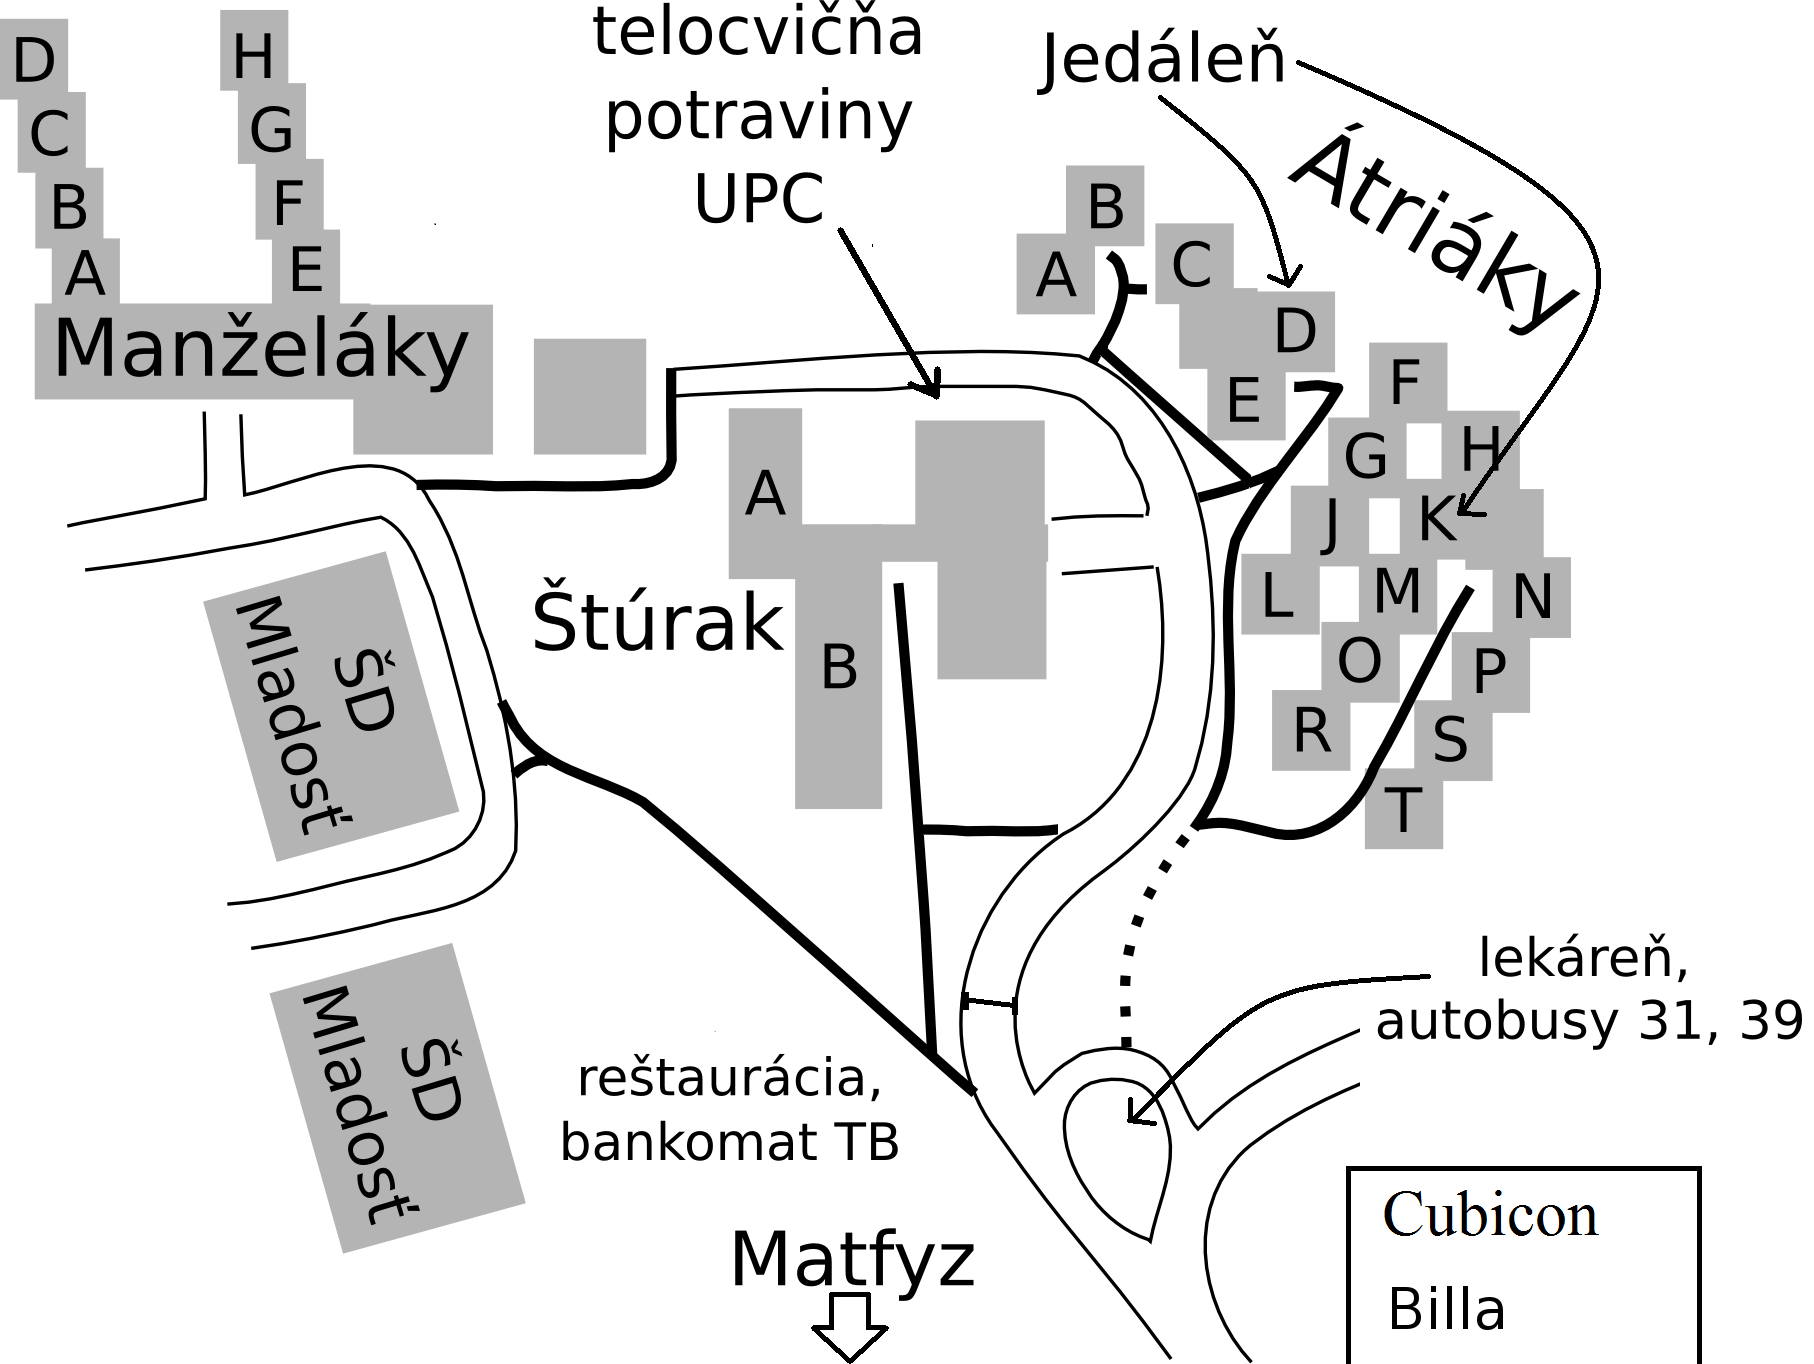
\includegraphics[width=1\textwidth]{obrazky/mapa-horiz_w}\label{fig:mapa-mlynov}
\par\end{centering}

\protect\caption{Mapa Mlynskej doliny}
\end{figure}

% TODO!!! dorobit pavilon S - DONE
\begin{figure}[h]
	\begin{centering}
		\vspace{-0.6cm}
		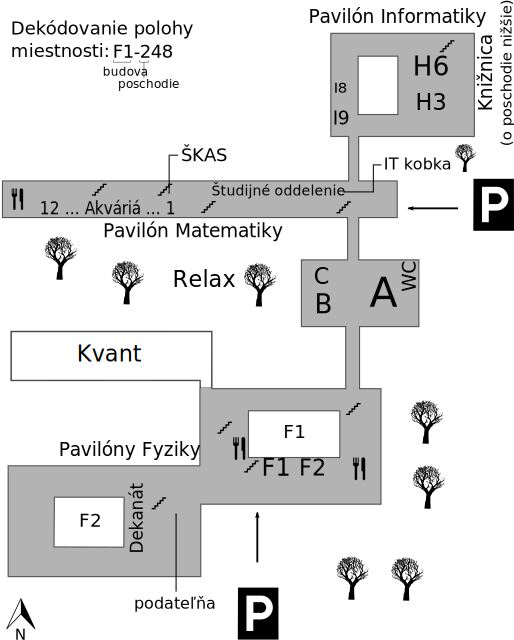
\includegraphics[width=1\textwidth]{obrazky/plan_matfyzu}\label{fig:mapa_fmfi}
		\par\end{centering}
	
	
	\protect\caption{Mapa FMFI}
	Online interaktívnu mapu aj s vyhľadávaním nájdeš na~\href{http://mapa.matfyzjein.sk}{\texttt{mapa.matfyzjein.sk}}, pre smartfóny s Androidom je k dispozícii v Google Play aplikácia ,,Sprievodca FMFI". Okrem označenia jednotlivých miestností (a kto v nej sedí), navigácie ,,z-do" v nej nájdeš aj denné menu v jedálňach.
\end{figure}

\begin{figure}[h!]
	\begin{centering}
		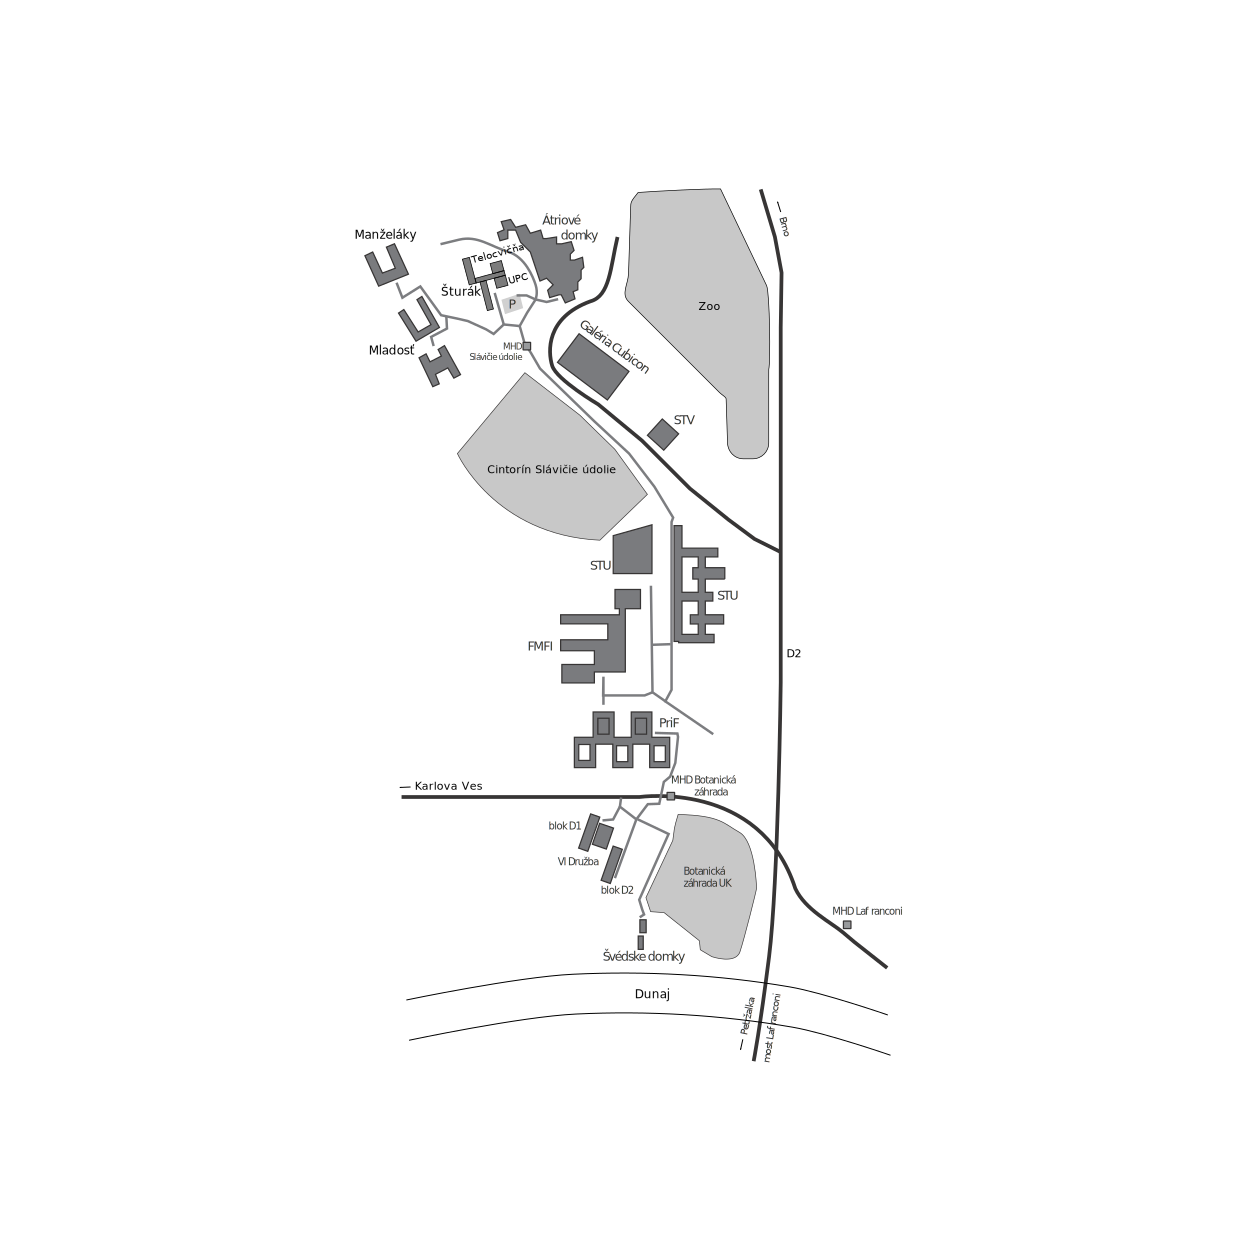
\includegraphics[width=1.8\textwidth,height=1.059\textheight,keepaspectratio]{obrazky/mapka_okolie_PriF}\label{fig:mapka_okolia_PriF}
		\par\end{centering}
	\protect\caption{Mapa širšieho okolia Mlynskej doliny}
\end{figure}






\clearpage

\newpage
~\vfill
\noindent\makebox[\textwidth]{\rule{\linewidth}{0.4pt}}
\noindent
{\small Pripravila:\\
Študentská komora Akademického senátu (ŠKAS)\\
Fakulta matematiky, fyziky a informatiky\\
Univerzita Komenského v Bratislave\\
\\
\href{https://zona.fmph.uniba.sk/skas}{\texttt{https://zona.fmph.uniba.sk/skas}}\\
\href{https://instagram.com/matfyz_skas}{\texttt{https://instagram.com/matfyz\_skas}}\\
\href{https://www.facebook.com/groups/347339742672275/?ref=share}{\texttt{https://www.facebook.com/groups/347339742672275/}}\\
\href{https://www.facebook.com/MatFyzJeIn}{\texttt{facebook.com/MatFyzJeIn}}\\
\href{https://instagram.com/matfyzjein}{\texttt{https://instagram.com/matfyzjein}}\\
\href{http://www.youtube.com/MatFyzJeIn}{\texttt{youtube.com/MatFyzJeIn}}\\
\href{mailto:skas@fmph.uniba.sk}{\texttt{skas@fmph.uniba.sk}}\\
}

\noindent
{\small Autori:\\
Kristián Valentín, Zuzana Cocuľová, Matúš Balogh,\\
Róbert Kysel, Estilla Alföldiová, Ján Hreha, Kristína Jablonická,
Kristína Tomová, Anna Buchholcerova, František Herman, Štefan Krakovský, Michal Švehlík, Júlia Pukancová, Andrej Badík, Otto Kohulák, Adam Štefunko, Boris Bobáľ


\noindent
\small
Vydanie pre akademický rok \akademickyRok.\\
Sadzba pomocou programu \LaTeX.\\
Ďalšie použité programy: LyX, Inkscape, GIMP.}


\end{document}

